\documentclass{article}

\usepackage[top=1in, bottom=1.5in, left=1.2in, right=1.2in]{geometry}
\usepackage{graphicx}
\usepackage{afterpage}
\usepackage{amsmath}


\title{\textbf{
    Média de pontos por temporada dos LA Lakers entre 1960 e 1991 vs 1992 e 2023
}}
\author{Grupo 8 - Gustavo Barroso Souza Cruz, Ian Cordibello Desponds}
\date{\today}


\begin{document}
    \maketitle
    \section*{Contexto}
    
    A NBA é a principal liga de basquete do mundo. Com o decorrer nos anos, a liga tem se tornado cada vez
    mais competitiva, com atletas mais preparados e apresentando uma tendencia tática de priorizazr a defesa
    tornando, assim, mais dificil ainda de pontuar contra os adversários. Com isso, estamos analisando se 
    a quantidade média de pontos durante as temporadas da NBA tem diminuido significativamente. Para isso,
    analisamos um de seus mais importantes times, o Los Angeles Lakers, nos períodos de 1960 a 1991 e de 1992 
    a 2023 e verificamos se a média mudou muito.\\
    \\

    \section*{A análise}

    \subsection*{Tratando os Dados}

    Ao tratar os dados da base de dados. Obtivemos que a média de pontos por temporada do Los Angeles Lakers 
    entre 1960 e 1991 foi de aproximadamente 113.22, enquanto entre os anos de 1992 e 2023 a média foi de
    aproximadamente 103.91.
    Assim ficaram as distribuições pra cada período:

    \begin{figure}[h]
        \centering
        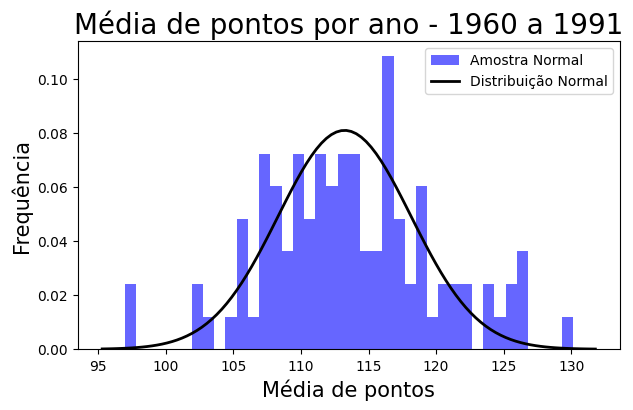
\includegraphics[width=0.49\textwidth]{pontos_60_91.png}
        \hfill
        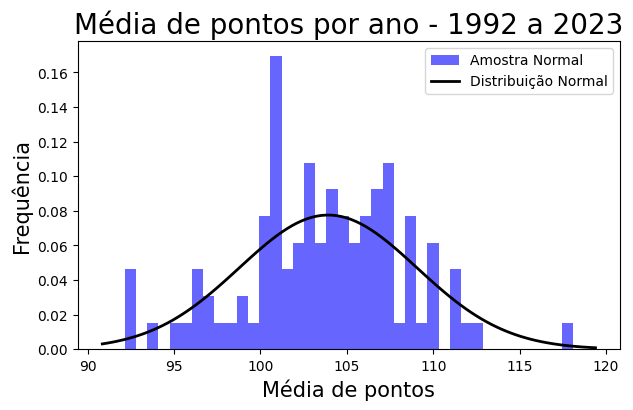
\includegraphics[width=0.49\textwidth]{pontos_92_23.png}
        \caption{Distribuição dos pontos do Los Angeles Lakers entre 1960-1991 e 1992-2023.}
    \end{figure}
    

    \subsection*{T-Teste}

    Ao realizar o T-Teste com as médias encontradas anteriormente, obtivemos um p-valor de aproximadamente
    $7.077 \times 10^{-10}$.


    \section*{Conclusão}

    Já que esperamos que a média de pontos tenha baixado significativamente, nossa hipótese nula $H_0$
    é que a média entre os períodos não é diferente e a hipótese alternativa $H_1$ é que a média do período
    de 1992 a 2023 ($\mu_1$) é menor que a média do período de 1960 a 1991 ($\mu_0$).\\
    
    Levando em conta que $\alpha = 0.05$, a partir do resultado obtido, podemos observar que, já que 
    $p-valor < \alpha$, falhamos em rejeitar a hipótese nula. O que não prova, porém sustenta nossa 
    hipótese alternativa.\\


    \section*{Autoavaliação - Conceito A}

    Nós acreditamos que merecemos o conceito A pois, seguindo a rubrica do trabalho, observamos um mesmo
    fenômeno em dois grupos (antes e depois de 1992) e, com as médias obtidas para cada grupo, fizemos
    e interpretamos o T-teste para verificar se as médias enre os grupos eram significativamente diferentes.
    Além disso, contextualizamos e explicamos o porquê de esperarmos uma mudança entre eles e construímos
    gráficos intuitivos para facilitar a visualização dos dados.\\


    \section*{Referências}

    [$1$] Dados do LAL  https://www.basketball-reference.com/teams/LAL/

\end{document}